\subsection{Applying Polya's Theorem}
We can use Polya's Theorem to count unlabeled graphs. 

\begin{definition}
    A \emph{graph} is a pair of sets $(V, E)$ where $V$ is the set of vertices
    and $E \subseteq V \times V$. 
\end{definition}

\begin{definition}
    Two graphs are isomorphic if there is a map $\pi : (V, E) \to (V_2, E_2)$
    such that $\pi(E) = \set{(\pi(v_1), \pi(v_2)) \, \forall (v_1, v_2) \in E} = E_2$
     and $\pi(V) = V_2$. 
\end{definition}

\begin{example}1
    These two graphs are isomorphic under the transformation $\pi = (1)(2)(34)$.
    \begin{center}
        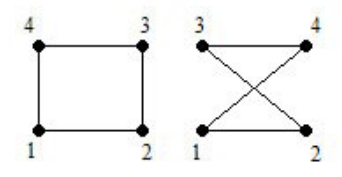
\includegraphics[scale=1]{figures/isomorphic_graphs.png}
    \end{center}
\end{example}

\begin{problem} 1
    Apply Polya's Theorem to count all graphs with $n = 3, 4$ vertices.
\end{problem}

For a graph with 3 vertices, we want to consider the cycle index polynomial 
for $S_3$: 
\begin{center}
    \begin{tabular}{|c|c|c|}
        \hline 
        $\pi$ & monomial & Action on edges \\ 
        (1)(2)(3) & $x_1^3$ & $(\ol{12})(\ol{13})(\ol{23})$ \\
        (1)(23) & $x_1x_2$ & $(\ol{12} \, \ol{13})(\ol{23})$ \\
        (2)(13) & $x_1x_2$ & $(\ol{21} \, \ol{23})(\ol{13})$ \\
        (3)(12) & $x_1x_2$ & $(\ol{31} \, \ol{32})(\ol{12})$ \\
        (123) & $x_3$ & $(\ol{12} \, \ol{23} \, \ol{31})$ \\ 
        (132) & $x_3$ & $(\ol{13} \, \ol{32} \, \ol{21})$ \\ \hline
    \end{tabular}
\end{center}
\[ P_{S_3^{(2)}} = \frac 16 (x_1^3 + 3x_1x_2 + 2x_3)\]
To enumerate, let the weight of an edge be $r$, and the weight of a lack of
edge be $b$, Thus, plugging in in accordance with the enumeration theorem,
\[
    P_{S_3} = \frac 16 ((r+b)^3 + 3(r+b)(r^2+b^2) + 2(r^3 + b^3)). 
\]
Because we don't care about lack of edges, let $b = 1$. Then this simplifies to 
\[ r^3 + r^2 + r + 1.\]
Next, let $r = 1$ so $x_i = 2$.
\[ P_3 = \frac 16 (2^3 + 3 \cdot 4 + 2 \cdot 2) = 4. \]
Now, let's do this for $S_4$: 
\begin{center}
    \begin{tabular}{|c|c|c|c|}
        \hline
        Number & form of $\pi$ & $S_4^{(2)}$ monomial & Action on edges \\ 
        $\binom 4 0 (1-1)!$ & (1)(2)(3)(4) & $x_1^6$ & $(\ol{12})(\ol{13})(\ol{14})(\ol{23})(\ol{24})(\ol{34})$ \\
        $\binom 4 2 (2-1)!$ & (1)(2)(34) & $x_1^2 x_2^2$ & $(\ol{12})(\ol{13}\,\ol{14})(\ol{23}\,\ol{24})(\ol{34})$ \\
        $\binom 4 3 (3-1)!$ & (1)(234) & $x_3^2$ & $(\ol{12}\,\ol{13}\,\ol{14})(\ol{23}\,\ol{34}\,\ol{42})$ \\
        $\binom 4 2 \cdot \frac 12$ & (12)(34) & $x_1^2 x_2^2$ & $(\ol{12})(\ol{23}\,\ol{14})(\ol{24}\,\ol{13})(\ol{34})$ \\
        $(4-1)!$ & (1234) & $x_2x_4$ & $(\ol{12}\,\ol{23}\,\ol{34}\,\ol{41})(\ol{13}\,\ol{24})$ \\
        \hline 
    \end{tabular}
\end{center}
Thus, 
\[ P_{S_4^{(2)}} = \frac 1{24} (x_1^6 + 9 x_1^2 + 8x_3^2 + 6 x_2 x_4). \]
Then, to enumerate, we let the weight of no edge be 1, and the weight of an edge be $x$, and get 
\[ x^6 + x^5 + 2x^4 + 3x^3 + 2x^2 + x + 1. \]
When we let $x = 1$, this simplifies to 11. 

We can also do this for $n = 5$ and higher $n$ as well, and the computations are similar. 